\documentclass[12pt, a4paper]{article}
\usepackage[utf8]{inputenc}
\usepackage{graphicx}
\usepackage{gensymb}
\usepackage{amsmath}
\usepackage{float}
\usepackage{subcaption}
\usepackage{caption}

\title{Differential methods for partial differential equations}
\author{Miha Pompe}
\date{January 2022}

\begin{document}
\begin{titlepage}
	\centering
 	
\includegraphics[width=0.45\textwidth]{logo_fmf_uni-lj_sl_veliki.png}\par\vspace{1cm}
	\vspace{1cm}
	\vspace{1.5cm}
	{\huge\bfseries Differential methods for partial differential equations\par}
	\vspace{2cm}
	{\Large Miha Pompe 28191072\par}
	\vfill
	\vfill
% Bottom of the page
	{\large January 2022\par}
\end{titlepage}
% \maketitle
\thispagestyle{empty}
\clearpage
\pagenumbering{arabic}
\newpage


\section{Introduction}

One-dimensional non-stationary Schrodinger's equation is the basic tool used to determine the time evolution of a quantum system in a given potential:
\begin{equation*}
  \left(i\hbar\frac{\partial}{\partial t}-H\right)\psi(x,t)=0,\quad H=-\frac{\hbar^2}{2m}\frac{\partial^2}{\partial x^2}+V(x)
\end{equation*}
In order to simplify the expression let $\hbar = m = 1$, which gives
\begin{equation*}
    H=-\frac{1}{2}\frac{\partial^2}{\partial x^2}+V(x)
\end{equation*}
To numerically compute the time and space evolution we'll use differential methods. For time evolution we know that
\begin{equation*}
  \psi(x,t+\Delta t)=e^{-i H \Delta t} \psi(x,t)\approx \frac{1-\frac{1}{2} i H \Delta t}{1+\frac{1}{2} i H \Delta t}\psi(x,t).
\end{equation*}
Let's discretize time into $N$ points ($[0, ..., N\Delta t]$) and space ($[a, ... , b]$). We will approximate spacial derivatives using finite differences:
\begin{equation*}
  \Psi''(x)\approx \frac{\psi(x+\Delta x,t)-2\psi(x,t)+\psi(x-\Delta x,t)}{\Delta x^2}=\frac{\psi_{j+1}^n - 2\psi_j^n+\psi_{j-1}^n}{\Delta x^2}\>.
\end{equation*}
Plugging this into Schrodinger's equation we get a system of equations which can be rewritten in matrix form
\begin{equation*}
  \mathsf{A}\boldsymbol{\Psi}^{n+1}=\mathsf{A}^\ast \boldsymbol{\Psi}^n,\qquad
  \mathsf{A}=\begin{pmatrix}
  d_1 & a \\
  a   & d_2 & a \\
  & a & d_3 & a \\
  & & \ddots & \ddots & \ddots \\
  & & & a & d_{N-2} & a \\
  & & & & a & d_{N-1}
  \end{pmatrix}\>,
\end{equation*}
where $\boldsymbol{\Psi}^n=(\psi_1^n,\ldots,\psi_{N-1}^n)^T$ and
\begin{equation*}
  b=i \frac{\Delta t}{2 \Delta x^2},\qquad a=-\frac{b}{2},\qquad d_j = 1+b+i \frac{\Delta t}{2}V_j\>.
\end{equation*}
To increase the accuracy of the method we can modify $\boldsymbol{A}$ matrix by including more points in finite differences.


\section{Coherent state}

The first problem we will be solving is a harmonic oscillator with the following initial condition
\begin{equation*}
  \Psi(x,0)=\sqrt{\frac{\alpha}{\sqrt{\pi}}} e^{-\alpha^2 (x-\lambda)^2/2}
\end{equation*}
where the potential is $V(x) = \frac{1}{2} k x ^2$. The analytical solution in natural coordinates, $\alpha = k^{1/4}$, $\omega = \sqrt{k}$, $\xi = \alpha x$ and $\xi_\lambda = \alpha \lambda$, is a coherent state
\begin{equation*}
  \psi(x,t)=\sqrt{\frac{\alpha}{\sqrt{\pi}}} \exp\left[-\frac12 \left(\xi-\xi_\lambda \cos\omega t\right)^2 - i \left(\frac{\omega t}{2}+\xi\xi_\lambda \sin\omega t - \frac14 \xi_\lambda^2 \sin 2 \omega t\right)\right]\>.
\end{equation*}

Using the differential method we can compute the evolution of this system, which is shown in Figure 1a. We can observe sinusoidal movement over time as we would expect from a classical pendulum. The color is equal to the squared norm of the function at that point.

Figure 1b shows the comparison of the analytical and numerical solutions. At $N = 500$ the maximum error was $0,06$. $N$ is the number of points in time and space interval. The absolute error increases with time, which can also be seen in Figure 1d, where the error rises with every turn. Figure 1d shows the maximum absolute error at each time point with respect to different $N$s. In all cases the error rises over time, but in cases with higher $N$s the rate of change is slower. At every turn we can observe a substantial drop in error.

The accuracy and stability of the solution is highly dependent on $N$. The latter is shown in Figure 1c where we are observing maximum values at each point in time. Analytically the height of the peaks should be constant over time, but we see that all approximations tend to deviate from that. The higher the number of points $N$ the slower the peaks diverge. 

The overall maximum absolute error drops exponentially with $N$ as can be observed from Figure 1e. Despite very high $N$ we are not able to achieve a very low relative error, at $N = 1000$ the relative error is around $8 \%$, therefore we can conclude that this method is not very accurate at realistic values of $N$.

The previous statement is confirmed in Figure 1e. The time complexity of solving the system rises polynomially with $N$. This is directly linked with computation of the inverse $\boldsymbol{A}$. A linear relation could be achieved using proper methods for solving banded matrices instead of using algorithms for arbitrary ones.

\begin{figure}[hbtp]
  \begin{subfigure}{0.5\textwidth}
  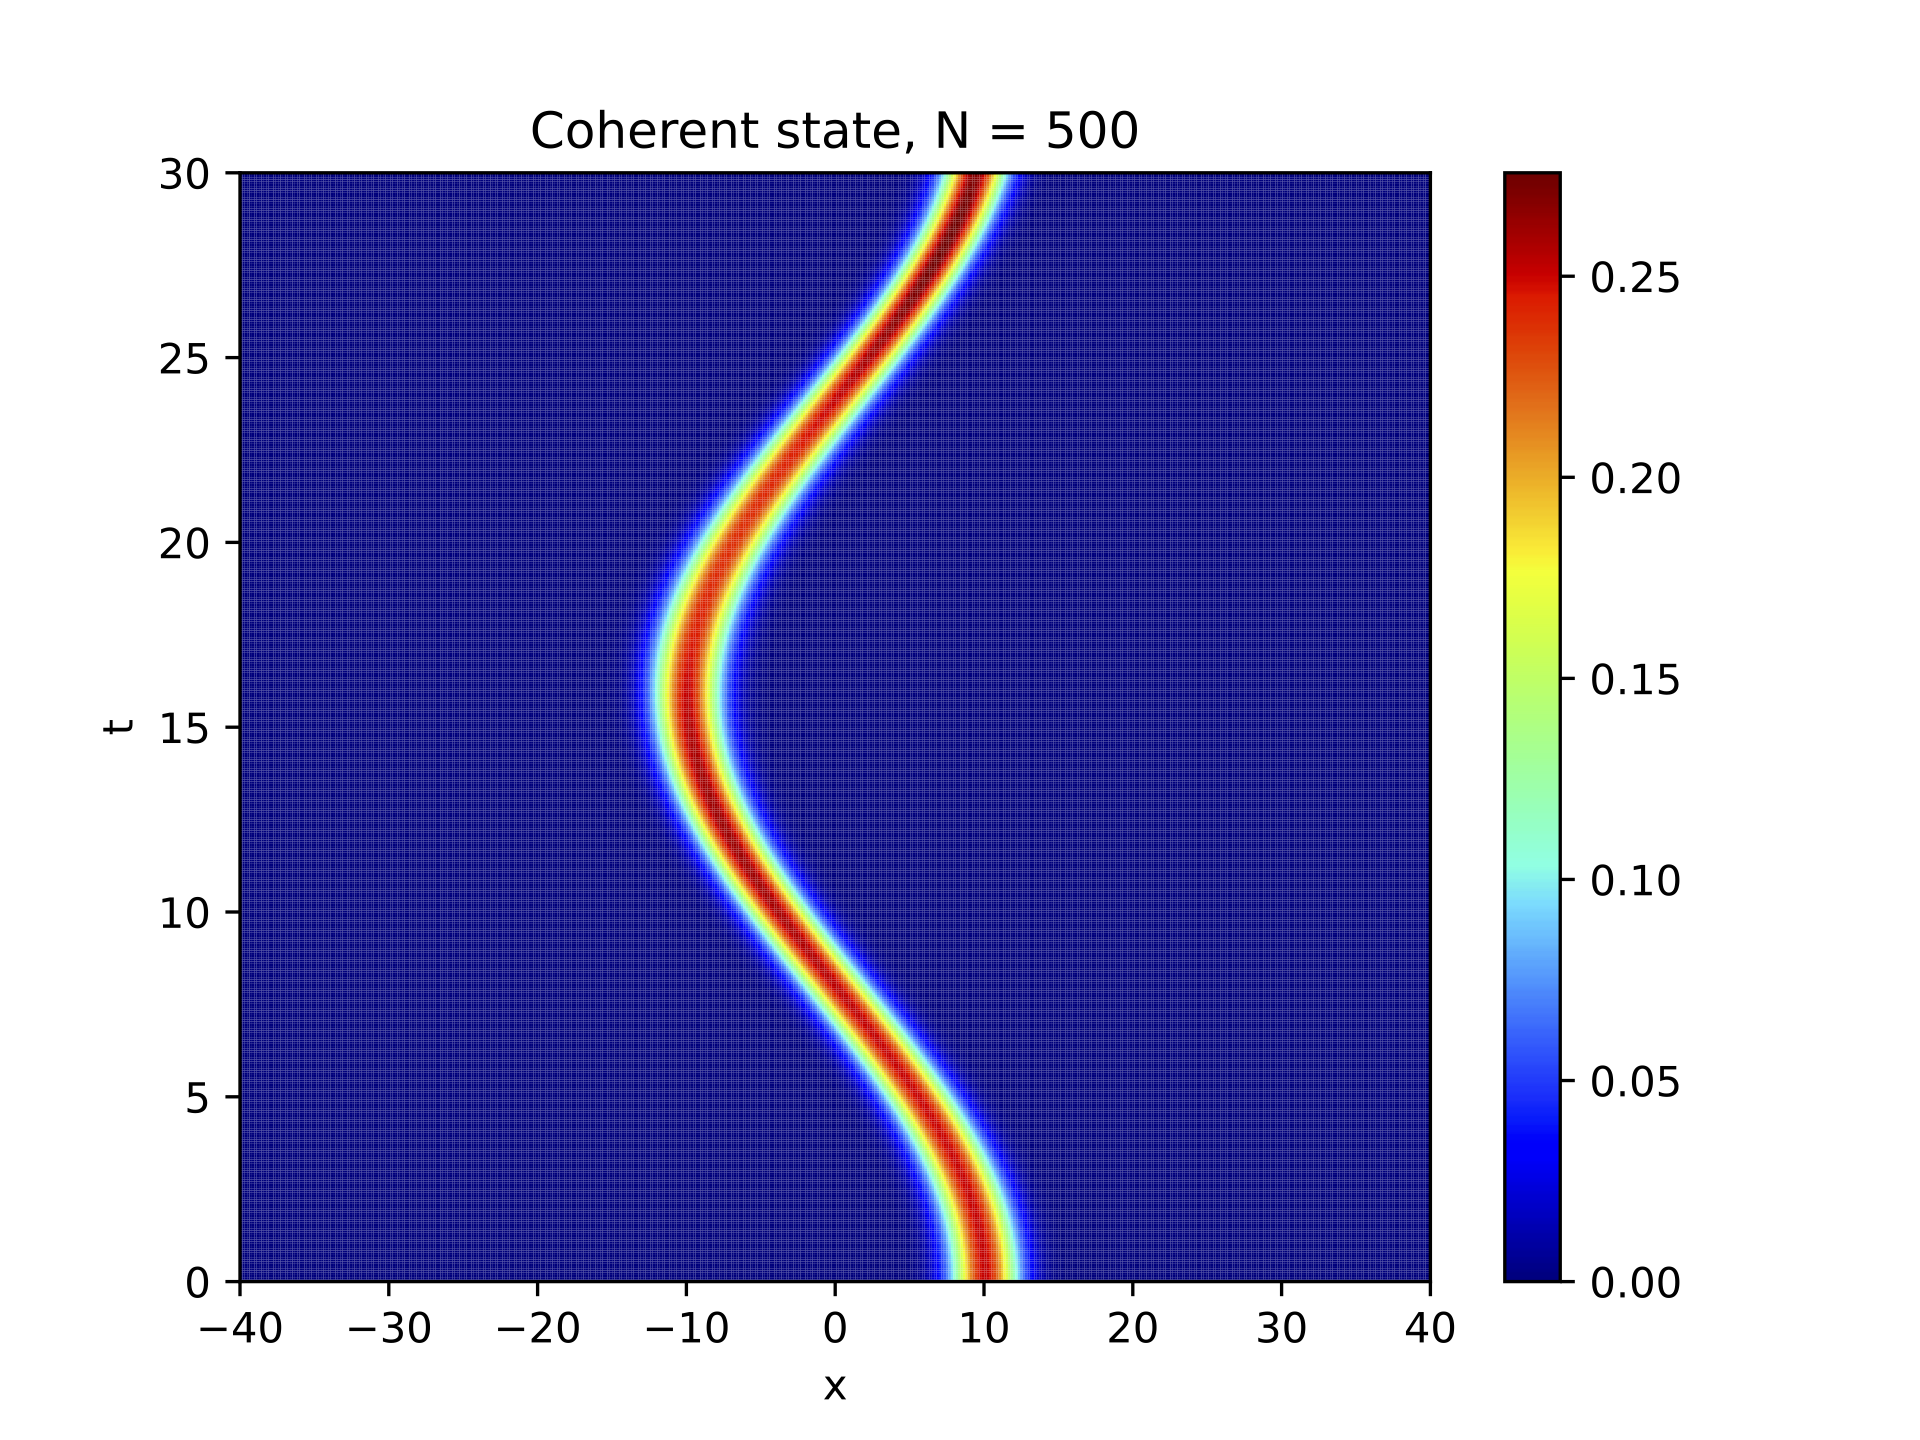
\includegraphics[width=\linewidth]{coherent copy.png}
  \caption{Coherent state solution} \label{fig:a}
  \end{subfigure}
  \hspace*{\fill}
  \begin{subfigure}{0.5\textwidth}
  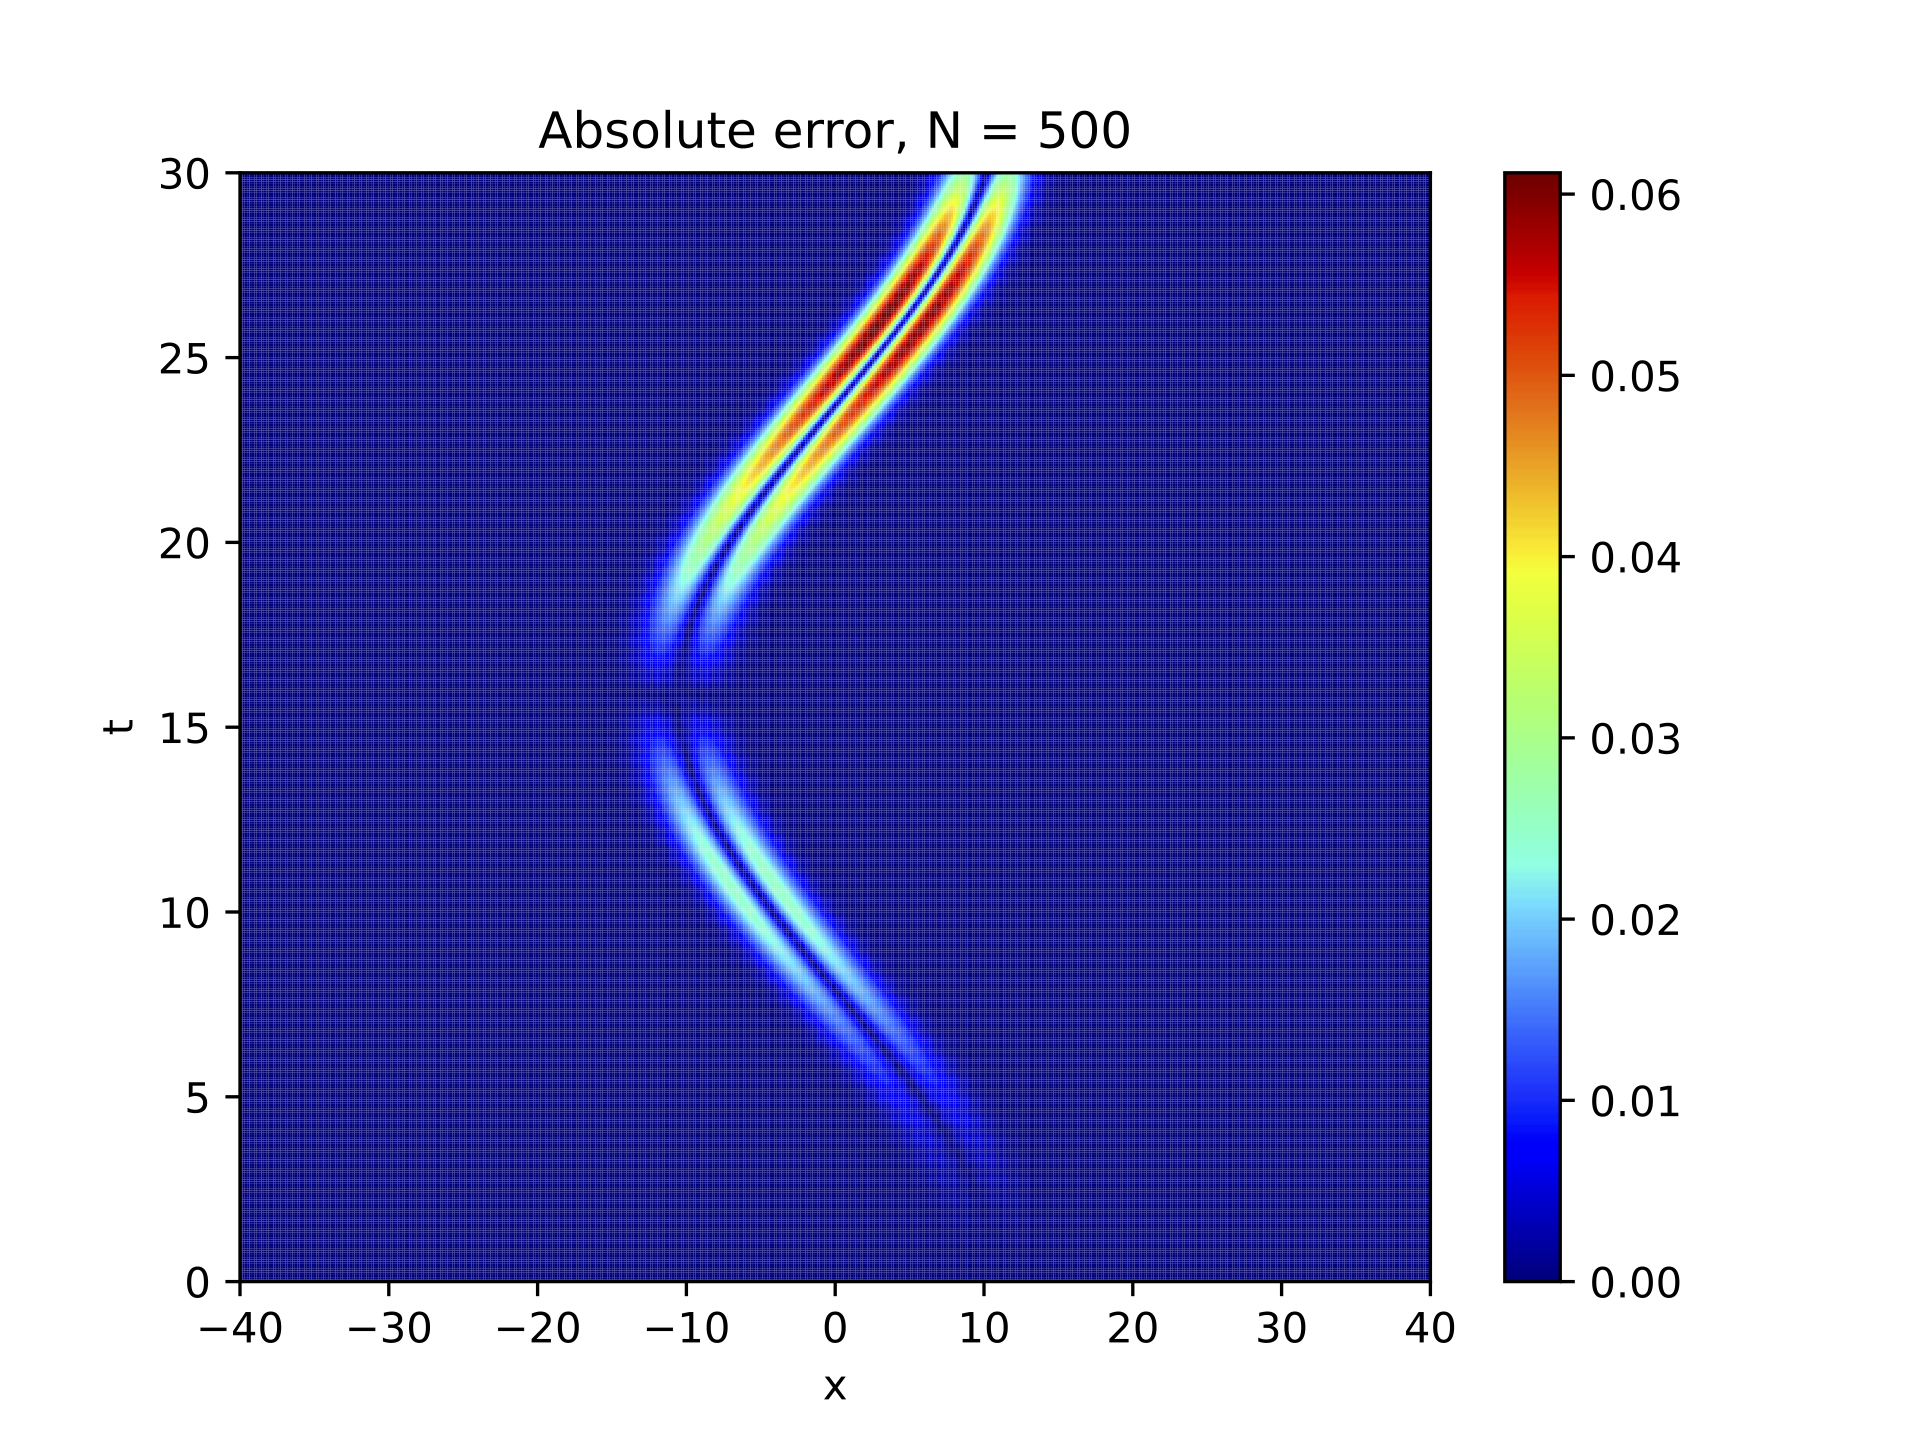
\includegraphics[width=\linewidth]{coherent_error copy.png}
  \caption{Absolute error of the numerical solution} \label{fig:b}
  \end{subfigure}
  \medskip
  \begin{subfigure}{0.5\textwidth}
  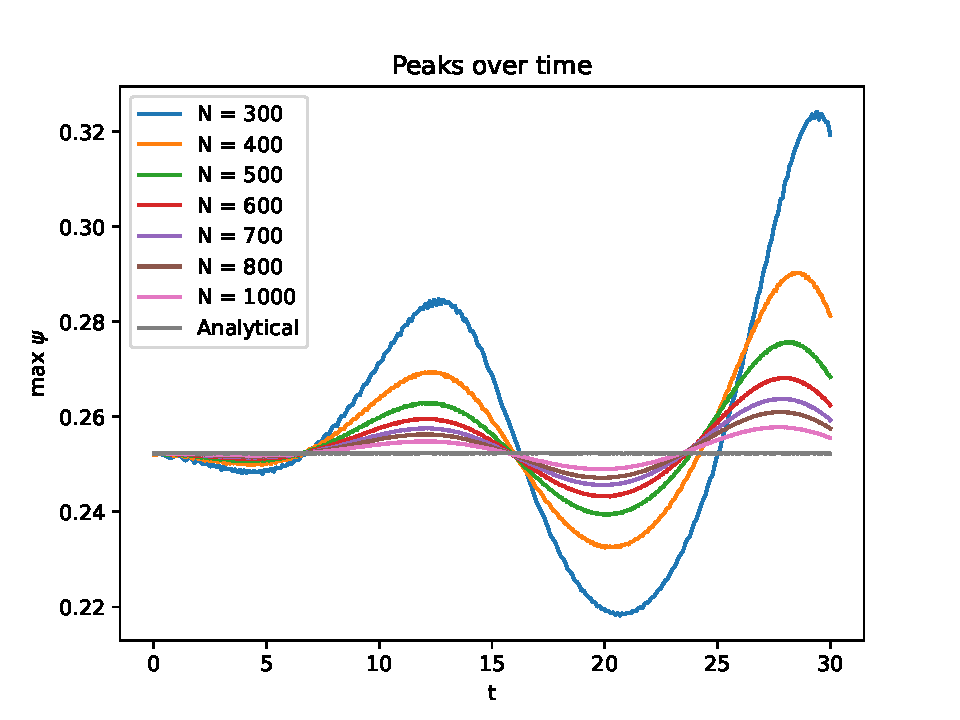
\includegraphics[width=\linewidth]{peaks.pdf}
  \caption{Solution peaks over time} \label{fig:c}
  \end{subfigure}
  \hspace*{\fill}
  \begin{subfigure}{0.5\textwidth}
  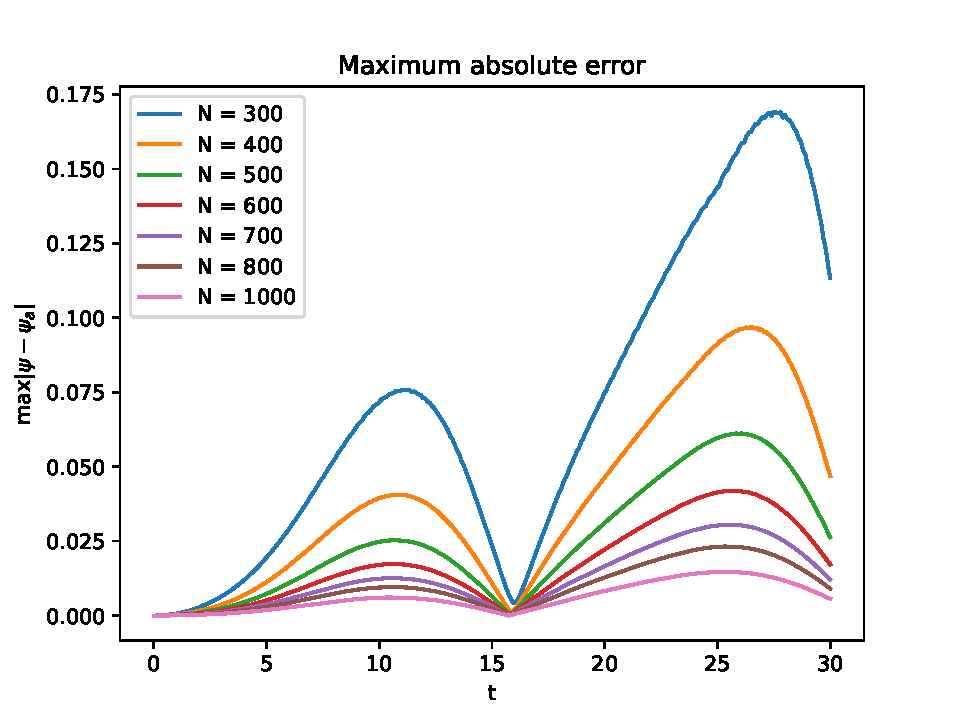
\includegraphics[width=\linewidth]{error_vs_time.pdf}
  \caption{Maximum error over time} \label{fig:d}
  \end{subfigure}
  \medskip
  \begin{subfigure}{0.5\textwidth}
  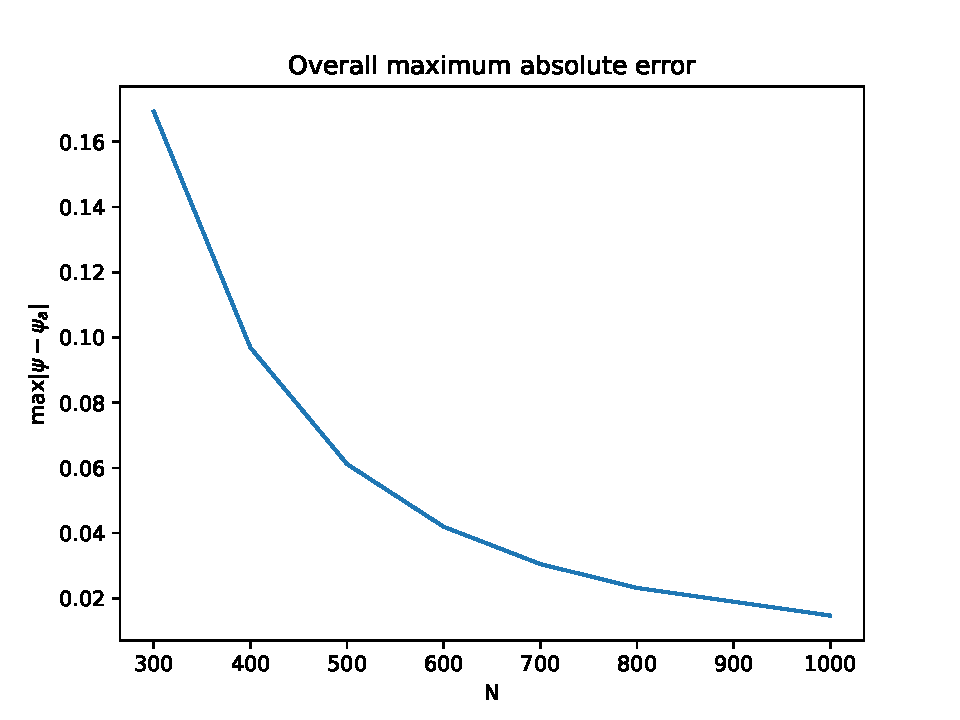
\includegraphics[width=\linewidth]{error_vs_N.pdf}
  \caption{Maximum error in relation to number of steps} \label{fig:c}
  \end{subfigure}
  \hspace*{\fill}
  \begin{subfigure}{0.5\textwidth}
  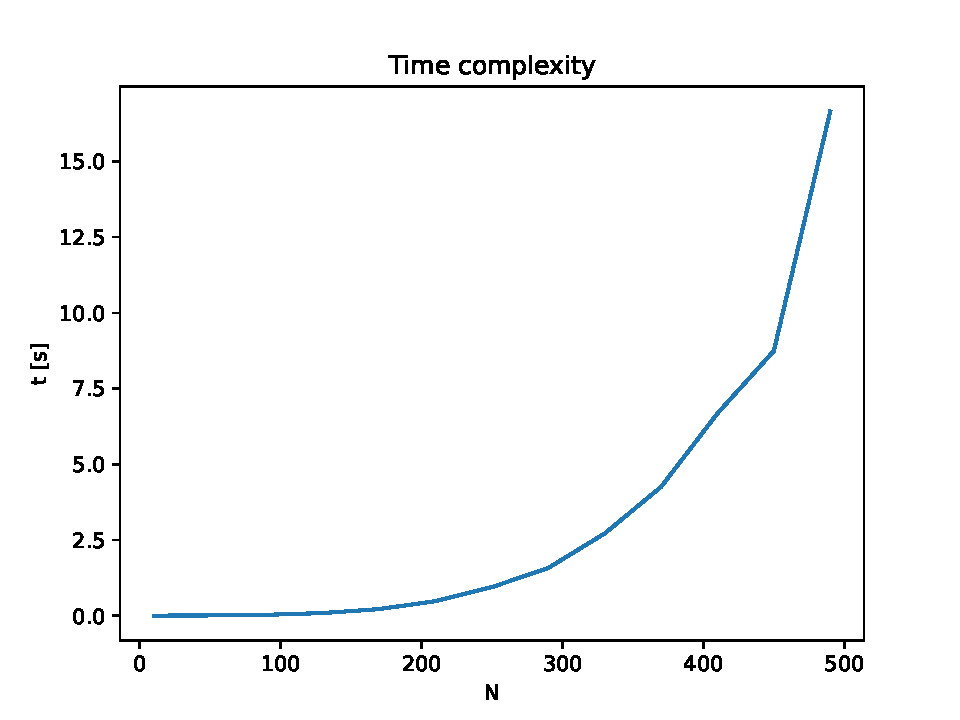
\includegraphics[width=\linewidth]{time_vs_N.pdf}
  \caption{Time complexity in relation to number of steps} \label{fig:d}
  \end{subfigure}
  \caption{Analysis of the coherent state solution and algorithm} \label{fig:1}
\end{figure}
 

\section{Gaussian wave packet}

The second initial problem is a Gaussian wave packet with no potential. The initial condition is given as
\begin{equation*}
  \psi(x,0)=(2\pi \sigma_0^2)^{-1/4} e^{i k_0(x-\lambda)}e^{-(x-\lambda)^2/(2\sigma_0)^2}
\end{equation*}
Analytical solution for this problem is
\begin{equation*}
  \psi(x,t)=\frac{(2\pi \sigma_0^2)^{-1/4}}{\sqrt{1+i t/(2\sigma_0^2)}} \exp\left[
    \frac{-(x-\lambda)^2/(2\sigma_0)^2+i k_0(x-\lambda)-i k_0^2 t/2}{1+i t/(2\sigma_0^2)}
    \right]
\end{equation*}
Plotting this solution gives us a packet traveling in one direction, whose width is slowly increasing.

\begin{figure}[hbtp]
  \begin{subfigure}{0.5\textwidth}
  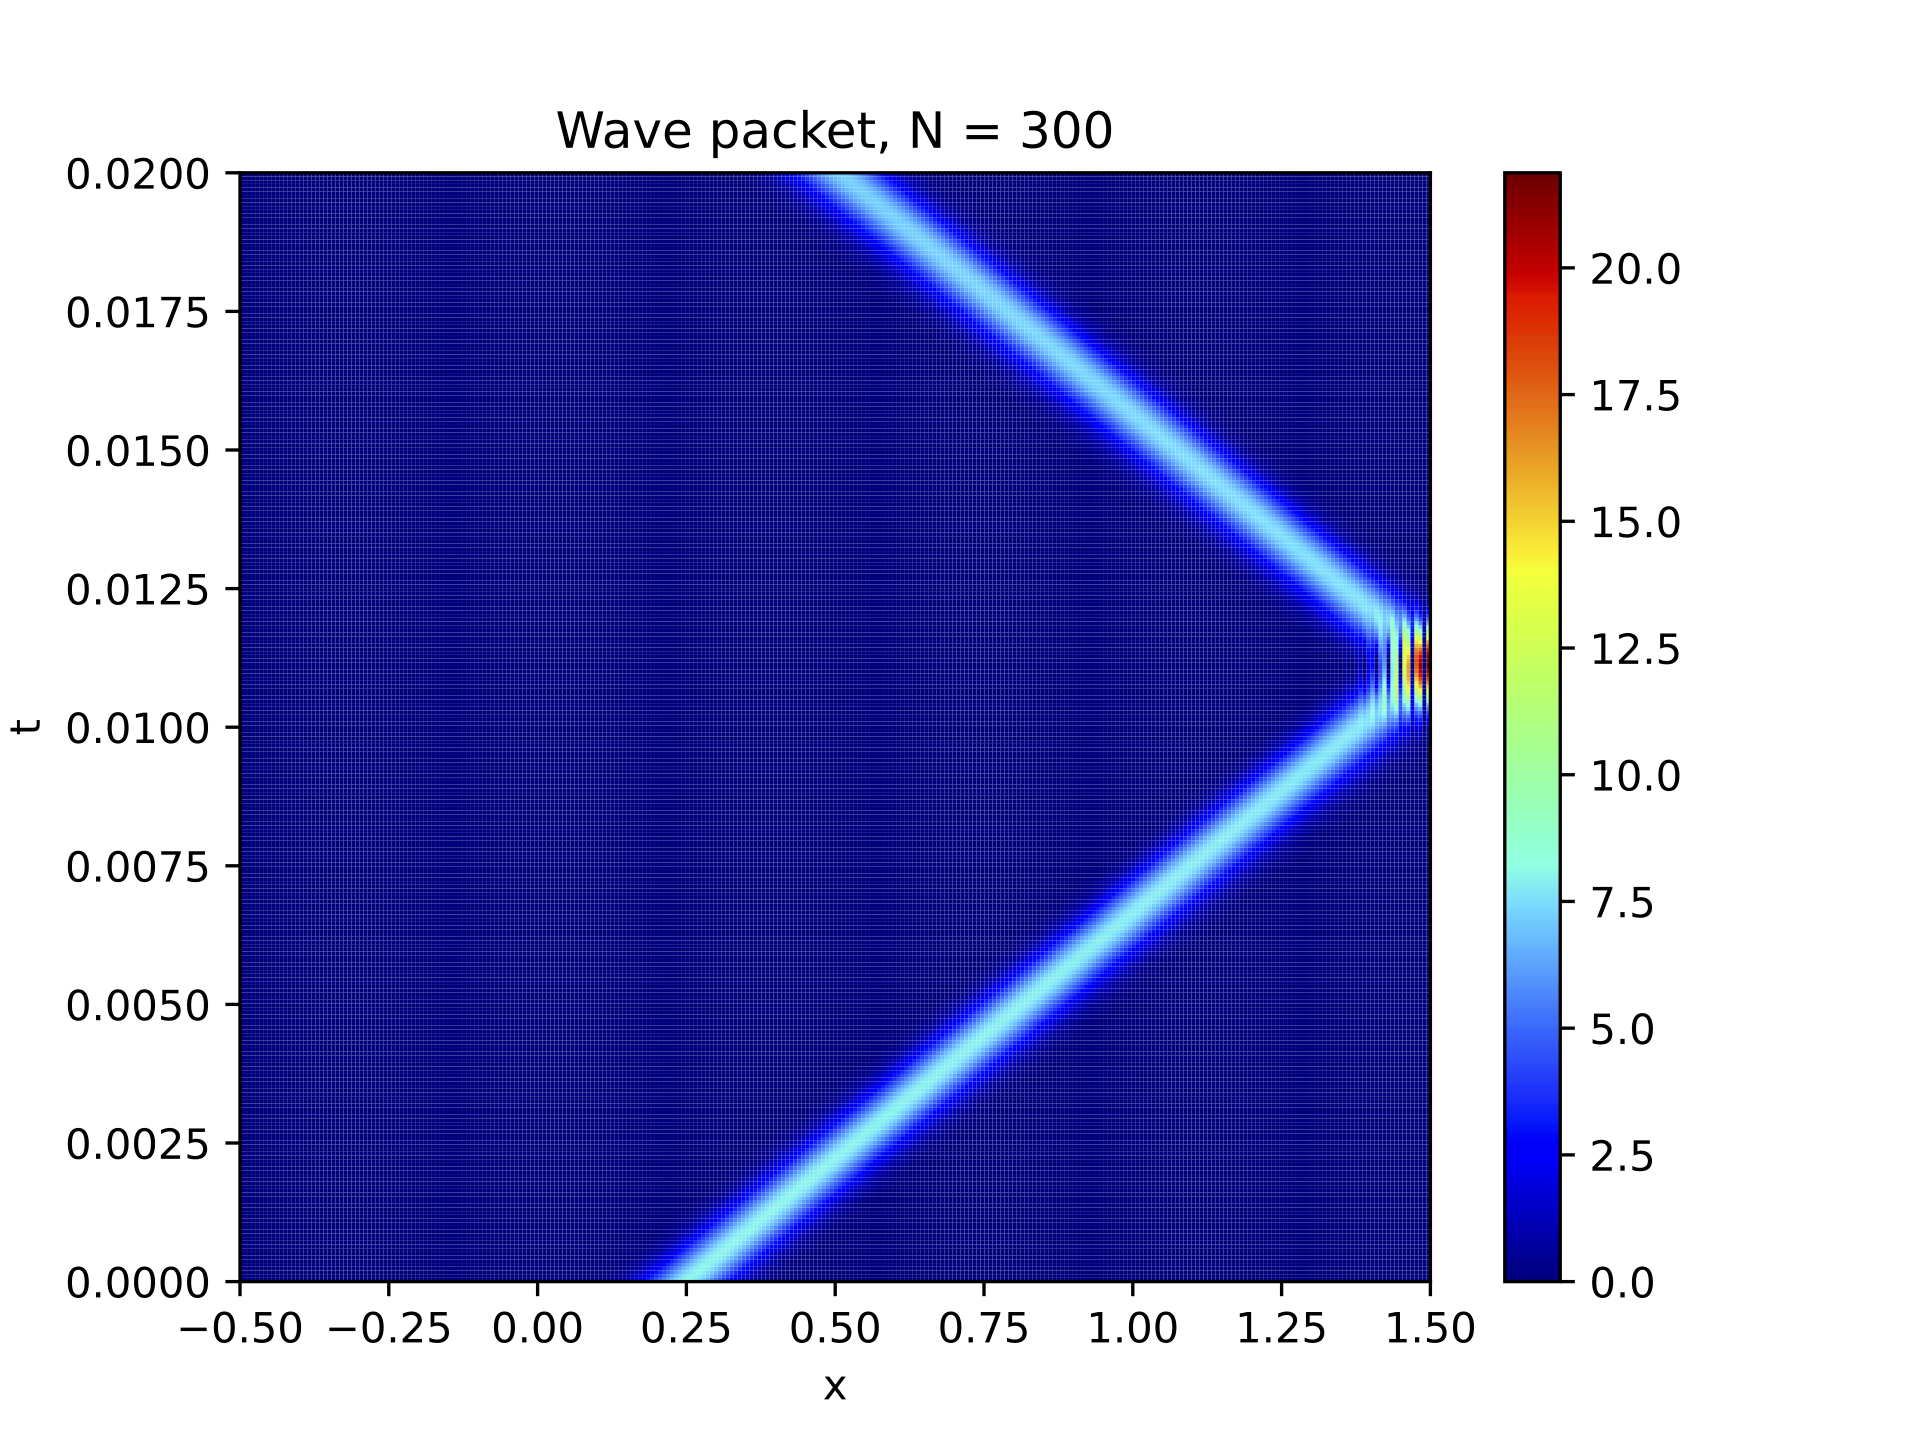
\includegraphics[width=\linewidth]{gauss_odboj copy.png}
  \caption{Wave packet solution} \label{fig:a}
  \end{subfigure}
  \hspace*{\fill}
  \begin{subfigure}{0.5\textwidth}
  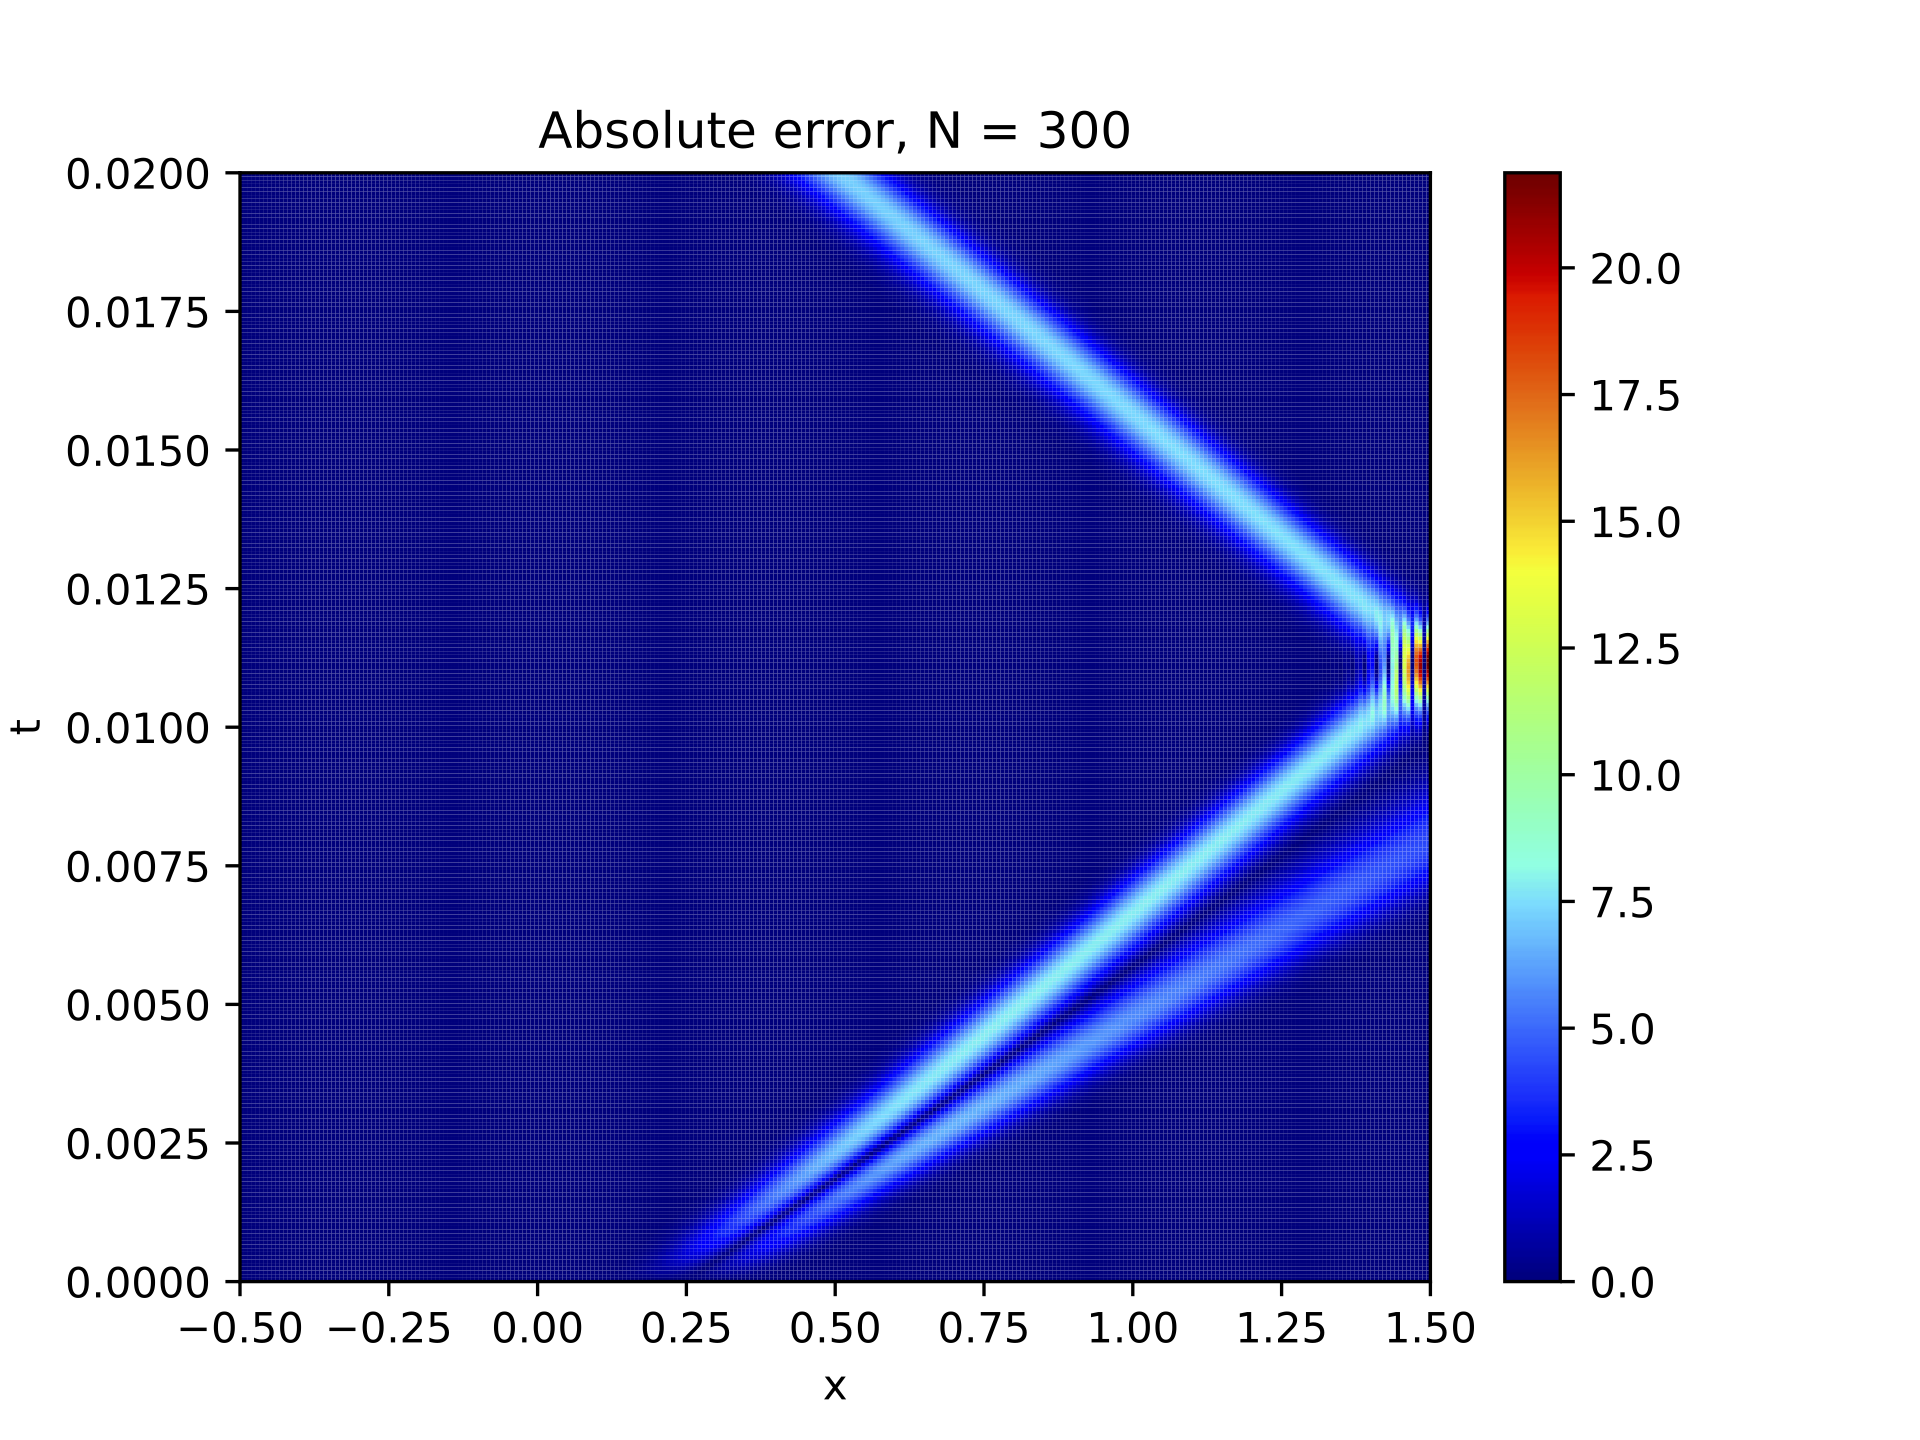
\includegraphics[width=\linewidth]{gauss_error_odboj copy.png}
  \caption{Absolute error of the numerical solution} \label{fig:b}
  \end{subfigure}
  \caption{Analysis of the Gaussian wave packet solution} \label{fig:1}
\end{figure}
 
Figure 2a shows the numerical solution to this problem and Figure 2b the deviation from the analytical solution. The deviations are relatively large, but after further inspection I presume these are the result of using to few division points $N$. I had also used the same amount of points for time and space. To improve these results a higher $N$ is needed and a more accurate method should be used. When the wave reaches the end of the interval it bounces of as if there was a potential barrier.

\newpage


\section{Method improvements}

As we have seen from previous results the method does not perform well in normal conditions. To improve it we can include more expansion factors. In time propagation we can use higher order Pade approximations, but this has not been examined in this work. The results of higher order spatial derivative approximations are shown in Figure 3. The approximation order is represented with $r$, $r \in {1, 2, 3, \dots}$, and is correlated to the number of side diagonals in matrix $\boldsymbol{A}$.

\begin{figure}[hbtp]
  \begin{subfigure}{0.5\textwidth}
  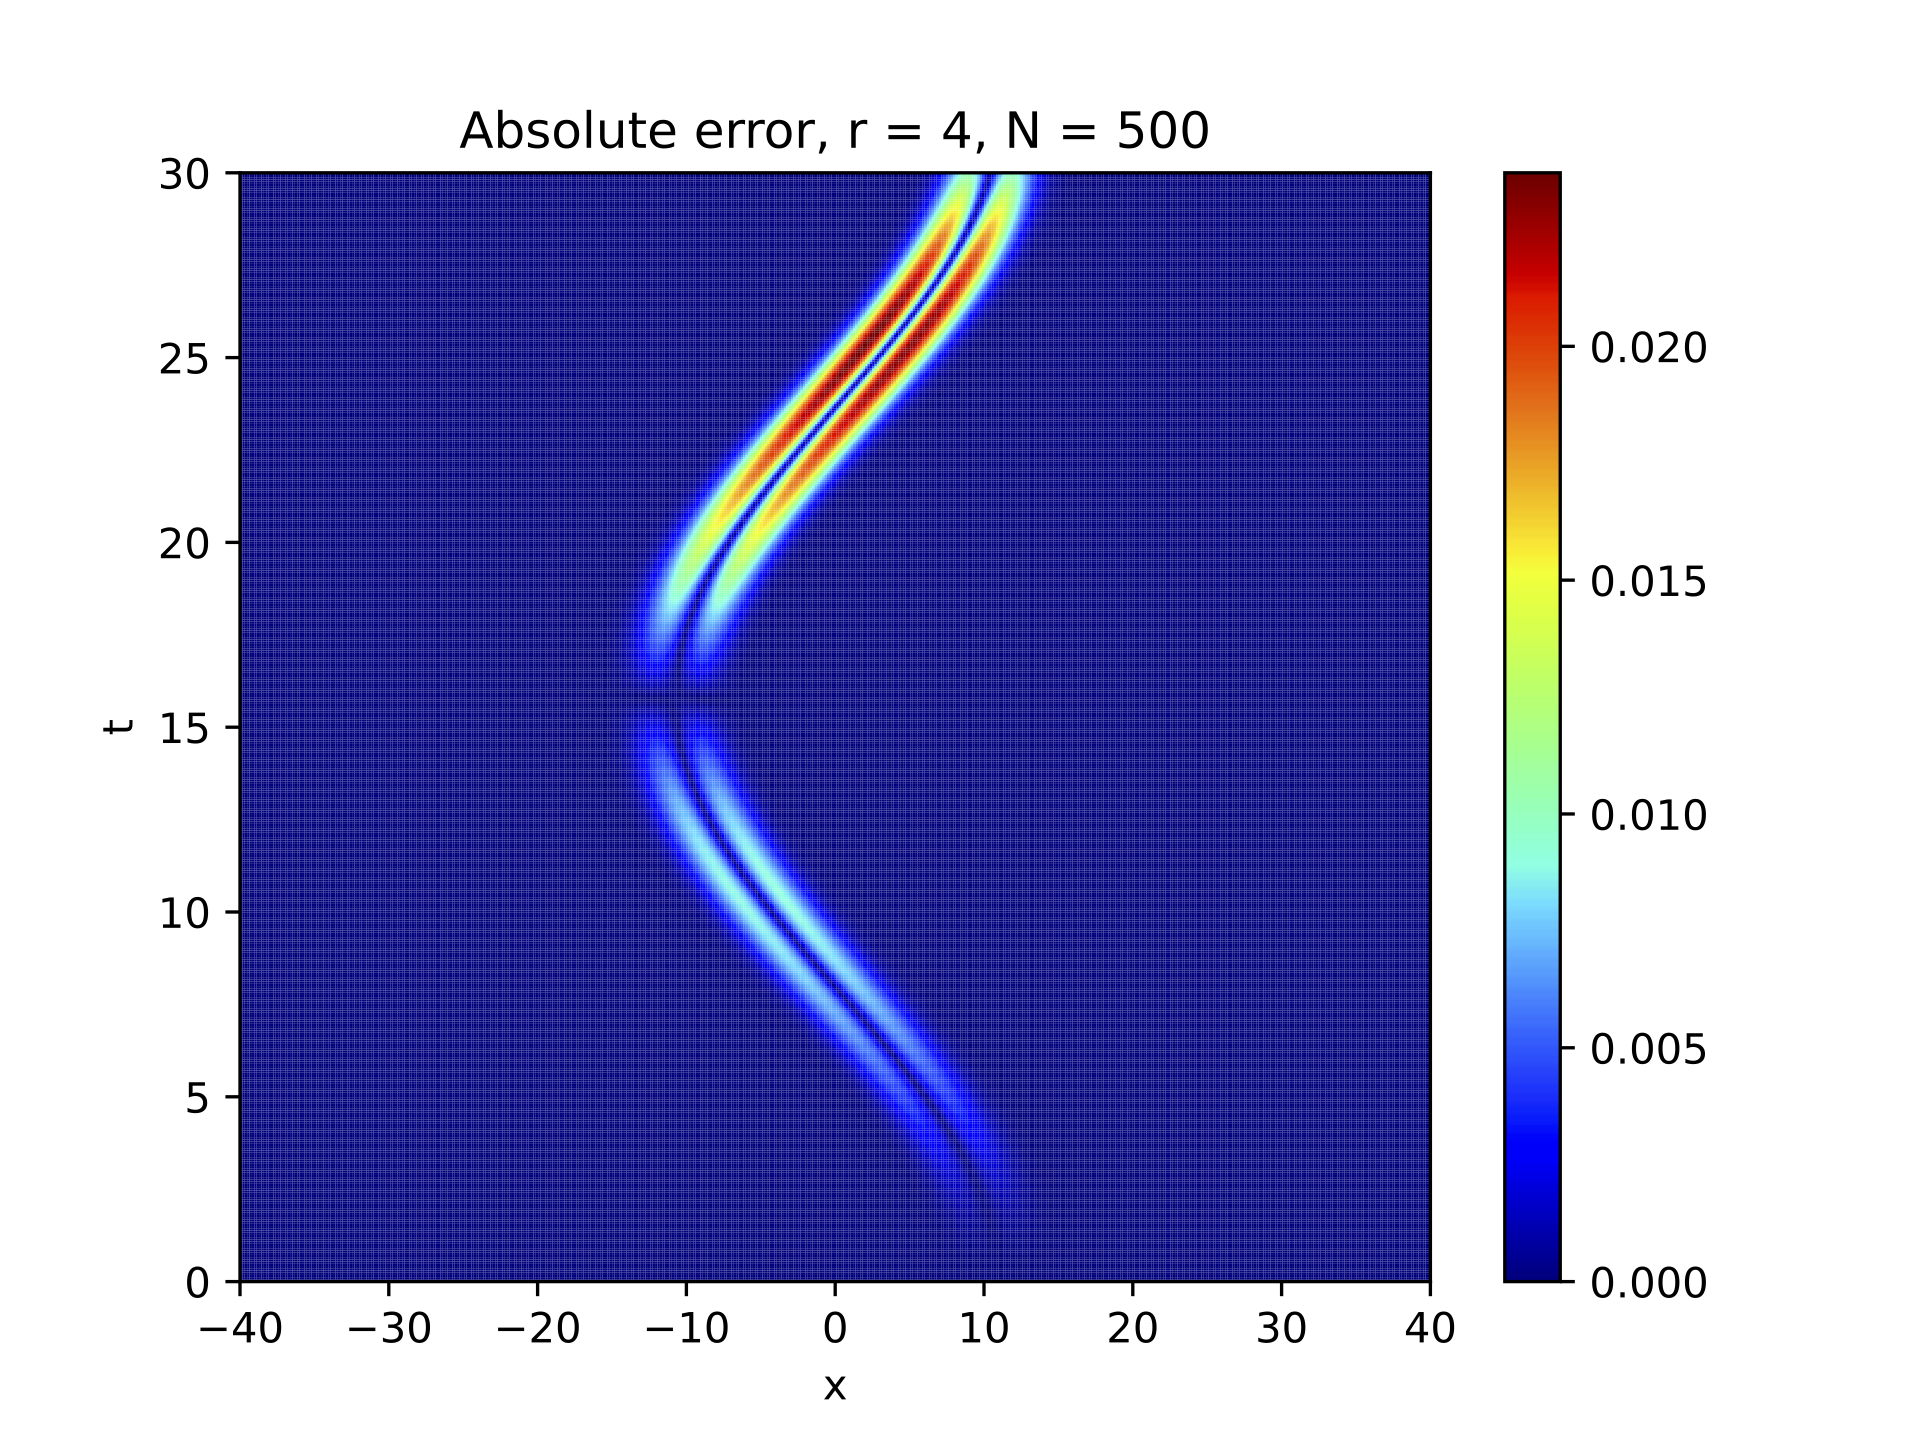
\includegraphics[width=\linewidth]{higher_r4 copy.png}
  \caption{Absolute error of the fourth order numerical solution} \label{fig:a}
  \end{subfigure}
  \hspace*{\fill}
  \begin{subfigure}{0.5\textwidth}
  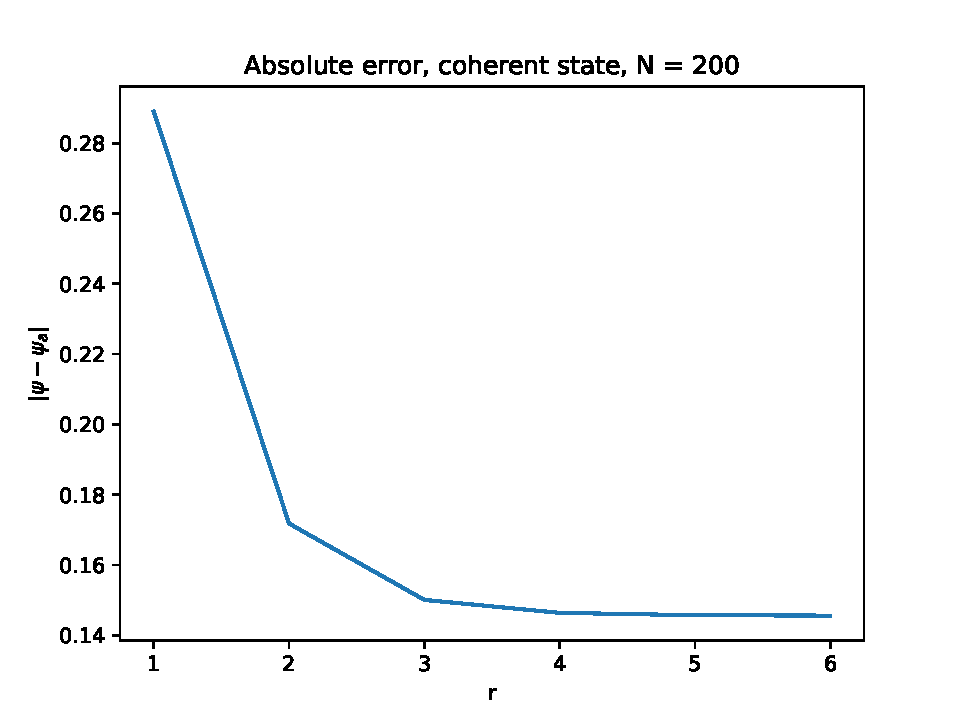
\includegraphics[width=\linewidth]{error_higher.pdf}
  \caption{Maximum absolute error in relation to approximation order} \label{fig:b}
  \end{subfigure}
  \caption{Analysis of the higher approximation method} \label{fig:1}
\end{figure}

Comparing Figure 1b and Figure 3a we notice that the maximum error dropped by around $60 \%$, by going from first to fourth approximation order. Figure 3b shows how the maximum error changes with higher orders with very few points ($N = 200$). By using higher order approximations we are able to use fewer division points and therefore decrease the computation time.

\end{document}